\documentclass{beamer}
\usetheme{Boadilla}
\usepackage{graphicx} % Required for inserting images
\usepackage{zx-calculus}
\usepackage{parskip}
\usepackage{braket}
\usepackage{amsmath}
\usepackage{booktabs}
\usepackage{tikz}
\usepackage{tikz-cd}
\usetikzlibrary{quantikz2}
\definecolor{USred}{cmyk}{0,1.00,0.65,0.34}
\usetikzlibrary{decorations.pathreplacing, calc}
\usepackage[style=numeric, backend=biber]{biblatex}
\addbibresource{referencias.bib}

\title{Quantum Protocols for Topological Codes with ZX Calculus}
\author{Salvador Márquez Grima}
\date{July 2026}

\begin{document}
\maketitle

\begin{frame}{Introduction}
    \begin{itemize}
        \item The  extreme fragility of quantum information requires the use of methods to detect and correct errors.
        \item Main difficulties: no-cloning theorem; measurement destroys information; and continuous errors.
        \item Solutions: Redundant encoding of information; multi-qubit parity operators; and discretization of errors
    \end{itemize}
    
\end{frame}

\begin{frame}{Quantum Error Correcting Codes}
\begin{itemize}
    \item We are encoding $k$ logical qubits into $n$ physical qubits, with $n>k$, by imposing some constraints on the physical qubits and thus defining a $2^k$-dimensional subspace of the total Hilbert space, called the code subspace. \cite{NielsenChuang2010}
    \item Errors push the state out of the code subspace. If each error corresponds to different undeformed and orthogonal subspaces, we can detect and correct them.
\end{itemize}
\end{frame}

\begin{frame}{Stabilizer Codes}
    \begin{definition}
        We define the n-dimensional Pauli group $\mathcal{P}_n$ as the set of all $n$-fold tensor products of Pauli matrices and the identity, with overall phases $\pm 1, \pm i$. A stabilizer is some abelian subgroup $ \mathcal{S} \subseteq \mathcal{P}_n$ that does not contain $-I$
    \end{definition}

The stabilizer can determine a code subspace, called the stabilizer code $C(\mathcal{S})$, as the set of all states that are fixed by the action of all elements of $\mathcal{S}$:
\begin{center}
    $C(\mathcal{S}) \equiv \{ \ket{\psi} \in \mathcal{H} : g \ket{\psi} = \ket{\psi}; \ \forall g \in \mathcal{S} \}$
\end{center}
\begin{alertblock}{Proposition}
If $\mathcal{S}$ is an Abelian subgroup of $\mathcal{P}_n$ that does not contain $-I$, then the code space $C(\mathcal{S})$ stabilized by $\mathcal{S}$ has dimension $2^{n - k}$, where $k$ is the number of independent generators of $\mathcal{S}$. \cite{Girvin2023}
\end{alertblock}
\end{frame}

\begin{frame}{Topological Codes}

    Consider a two-dimensional lattice embedded in a closed surface, with physical qubits attached to each edge. We can define a chain complex of vector spaces over $\mathbb{Z}_2$ by constructing the standard sets of $i$-chains $C_i$ for $i=0,1,2$, where the basis elements are the vertices, edges, and faces of the lattice. The boundary operators $\partial_i: C_i \to C_{i-1}$ are defined as usual. \cite{bombin2013introductiontopologicalquantumcodes}

    We can identify elements of the computational basis with 1-chains on the lattice $\ket{c} = \bigotimes_i \ket{c_i}$, where the field of coefficients is $\mathbb{Z}_2$. Homomorphisms from $C_1$ to $\mathcal{P}_n$ are defined as follows:
\begin{center}
    $X_c = \bigotimes_i X^{c_i}_i \quad \text{and} \quad Z_c = \bigotimes_i Z^{c_i}_i.$
\end{center}

\end{frame}
\begin{frame}    
\begin{figure}
\centering
\input{tikz/surfacecode.tex}
\label{fig:surface_code}
\end{figure}

The stabilizer generators are:
\begin{align*}
    X_f:= \prod _{e \in \partial_2 f} X_e \quad \text{and} \quad Z_v := \prod _{e |v \in \partial_1 e} Z_e
\end{align*}

\end{frame}

\begin{frame}{Surface Codes with Boundaries}
    
    \begin{figure}
        \centering
        \input{tikz/planarpatch.tex}
        \label{fig:surface_code_boundaries}
    \end{figure}
    
Top and bottom edges are closed boundaries, left and right edges are open boundaries. \cite{bravyi1998quantumcodeslatticeboundary}

\end{frame}

\begin{frame}{Transversal Operations with Planar Surface Codes: Lattice Surgery}
    \begin{figure}
        \centering
        
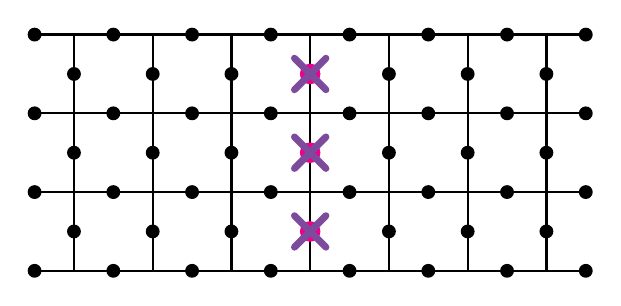
\begin{tikzpicture}[scale=1.0]
    % Define styles for nodes and edges
    \tikzset{
        blacknode/.style={circle, fill=black, inner sep=0pt, minimum size=5pt},
        pinknode/.style={circle, draw=magenta, fill=magenta, inner sep=0pt, minimum size=7pt},
        edge/.style={draw=black, thick}
    }
        \definecolor{crosscolor}{RGB}{125,75,155} % Purple

    % ==========================================
    % LEFT LATTICE
    % ==========================================
    % 1. Draw the underlying grid
    % Horizontal lines (x=0 to 3)
    \foreach \y in {0, 1, 2, 3} { \draw[edge] (-0.5,\y) -- (3,\y); } 
    % Vertical lines (x=0 to 2)
    \foreach \x in {0, 1, 2} { \draw[edge] (\x,0) -- (\x,3); } 

    % 2. Place black balls in the middle of horizontal edges
    \foreach \y in {0, 1, 2, 3} {
        \foreach \x in {-0.5, 0.5, 1.5, 2.5} {
            \node[blacknode] at (\x, \y) {};
        }
    }
    % 3. Place black balls in the middle of vertical edges
    \foreach \x in {0, 1, 2} {
        \foreach \y in {0.5, 1.5, 2.5} {
            \node[blacknode] at (\x, \y) {};
        }
    }

    % ==========================================
    % RIGHT LATTICE
    % ==========================================
    % Shifted left so it meets the left lattice perfectly
    
    % 1. Draw the underlying grid
    % Horizontal lines (x=3 to 6) - Now touching the left lattice at x=3
    \foreach \y in {0, 1, 2, 3} { \draw[edge] (3,\y) -- (6.5,\y); } 
    % Vertical lines (x=4 to 6)
    \foreach \x in {3, 4, 5, 6} { \draw[edge] (\x,0) -- (\x,3); } 

    % 2. Place black balls in the middle of horizontal edges
    \foreach \y in {0, 1, 2, 3} {
        \foreach \x in {3.5, 4.5, 5.5, 6.5} {
            \node[blacknode] at (\x, \y) {};
        }
    }
    % 3. Place black balls in the middle of vertical edges
    \foreach \x in {4, 5, 6} {
        \foreach \y in {0.5, 1.5, 2.5} {
            \node[blacknode] at (\x, \y) {};
        }
    }

    % ==========================================
    % CENTRAL PINK COLUMN
    % ==========================================
    % Placed precisely at x=3, sitting right on top of the touching horizontal edges
    \foreach \y in {0.5, 1.5, 2.5} {
        \node[pinknode] at (3, \y) {};
    }

        \foreach \y in {0.5, 1.5, 2.5} {
        \draw[crosscolor, line width=2.5pt, line cap=round] (3-0.2, \y-0.2) -- (3+0.2, \y+0.2);
        \draw[crosscolor, line width=2.5pt, line cap=round] (3-0.2, \y+0.2) -- (3+0.2, \y-0.2);
    }

\end{tikzpicture}
        \label{fig:surface_code_transversal}
    \end{figure}
    Representation of a rough splitting operation on a planar surface code. The initial state is $\ket{0}_L$ and the final state is $\ket{00}_L$.
    
\end{frame}

\begin{frame}
    \begin{figure}
        \centering
        \input{tikz/rough_merging.tex}
        \label{fig:surface_code_transversal}
    \end{figure}

Truth table for a rough merging operation on a planar surface code.    
\[
\begin{array}{cc|c}
\textcolor{blue}{\text{In}(1)} & \textcolor{blue}{\text{In}(2)} & \textcolor{blue}{\text{Out}} \\
\hline
0 & 0 & 0 \\
0 & 1 & 1 \\
1 & 0 & 1 \\
1 & 1 & 0 \\
\end{array}
\]
\end{frame}

\begin{frame}
Kraus operators for a rough merging operation on a planar surface code:
    \begin{equation*}
    M_R(\rho) = K_{0,R} \rho K_{0,R}^\dagger + K_{1,R} \rho K_{1,R}^\dagger 
    \end{equation*}
\begin{equation*}
K_{0,R} = \ket{+}_M \bra{++} + \ket{-}_M \bra{--} \quad K_{1,R} = \ket{+}_M \bra{+-} + \ket{-}_M \bra{-+}
\end{equation*}
Kraus operator for a rough splitting operation on a planar surface code:
\begin{equation*}
    U_R = \ket{++} \bra{+} + \ket{--} \bra{-}
\end{equation*}
\end{frame}


\begin{frame}{ZX Calculus}
\begin{align*}
    \zx{ \leftManyDots{n} \zxZ{\alpha} \rightManyDots{m}} &= \ket{\underbrace{0 \cdots 0}_{m}} \bra{\underbrace{0 \cdots 0}_{n}} + e^{i \alpha} \ket{{\underbrace{1 \cdots 1}_{m}}} \bra{\underbrace{1 \cdots 1}_{n}} \\
    \zx{\leftManyDots{n} \zxX{\alpha} \rightManyDots{m}} &= \ket{\underbrace{+ \cdots +}_{m}} \bra{\underbrace{+ \cdots +}_{n}} + e^{i \alpha} \ket{{\underbrace{- \cdots -}_{m}}} \bra{\underbrace{- \cdots -}_{n}}
\end{align*}
    
\begin{figure}
    \centering
    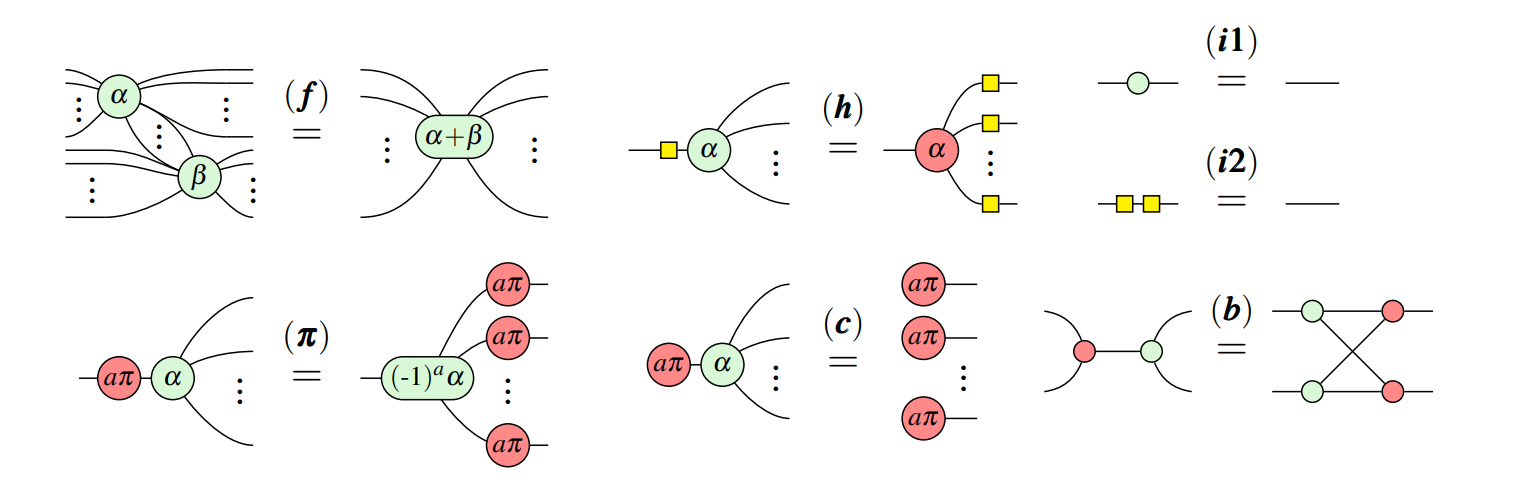
\includegraphics[width=\textwidth]{figures/Rewrite_Rules.png}
\end{figure}
Rewrite rules for ZX calculus as presented in \cite{KissingerWetering2024Book}.
\end{frame}


\begin{frame}{ZX Calculus and Lattice Surgery}

Correspondence between ZX diagrams and the Kraus operators of a lattice merging operation \cite{deBeaudrap2020}:

\begin{align*}
\begin{ZX}
\zxN{} \rar & \zxZ{} \rar & \zxN{} \\
\zxN{} \ar[ru] &          &
\end{ZX}
\ =& \ K_{0,S} \quad \quad
\begin{ZX}
\zxN{} \rar & \zxX{} \rar & \zxN{} \\
\zxN{} \ar[ru] &          &
\end{ZX}
\ = \ K_{0,R} \\
\begin{ZX}[phase in label below]
\zxN{} \rar & \rar           & \zxZ{} \rar & \zxN{} \\
\zxN{} \rar & \zxX{\pi} \ar[ru] &          &
\end{ZX}
\ =& \ K_{1,S} \quad \quad
\begin{ZX}[phase in label below]
\zxN{} \rar & \rar              &  \zxX{} \rar & \zxN{} \\
\zxN{} \rar & \zxZ{\pi} \ar[ru] &              &
\end{ZX}
\ = \ K_{1,R}
\end{align*}

Correspondence between ZX diagrams and the Kraus operators for a lattice splitting operation:

\begin{equation*}
\begin{ZX}
    \zxN{} & \zxZ{} \ar[r,start anchor=south,end anchor=south] & \zxNoneDouble|{}
\end{ZX} \
= \ U_S
\quad \quad
\begin{ZX}
    \zxN{} & \zxX{} \ar[r,start anchor=south,end anchor=south] & \zxNoneDouble|{}
\end{ZX}
\ = \ U_R
\end{equation*}
\end{frame}

\begin{frame}{Logical Verification and Optimization of Quantum Protocols}
    \begin{itemize}
        \item The rewrite rules of ZX calculus can simplify complex diagrams, conserving the represented linear map and allowing for the logical verification of quantum protocols.
        \item The simplification of ZX diagrams can also lead to the optimization of quantum protocols, reducing the number of operations and resources required for their implementation.
    \end{itemize}
\end{frame}

\begin{frame}{Quantum Protocols with ZX Calculus}
    \begin{itemize}
        \item Quantum Teleportation.
        \item CHSH Game.
        \item Magic Square Game.
    \end{itemize}
    
\end{frame}

\begin{frame}{CHSH Game}
    CHSH game is a problem in information theory that can be modeled as a non-local cooperative game \cite{watrous2025understandingquantuminformationcomputation}. Alice and Bob receive each a classical bit of information, $x$ and $y$, and they must produce a classical bit of information, $a$ and $b$, respectively, such that they satisfy the winning condition $a \oplus b = x \cdot y$. $P_{classic} \leq 0.75$.
    \begin{figure}
        \centering
        \input{tikz/CHSH_circuit.tex}
        \label{fig:chsh_game}
    \end{figure}
\end{frame}

\begin{frame}{CHSH Game in ZX Calculus}
    \begin{figure}
        \centering
        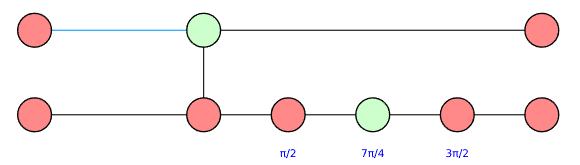
\includegraphics[width=\textwidth]{figures/CHSH1.png}
        \label{fig:chsh_game_zx}
    \end{figure}
    ZX diagram for the CHSH game with $(x,y) = (0,0)$ and $(m_0, m_1) = (0,0)$. The amplitude for each branch:

    \begin{equation*}
    \mathcal{A}_{x,y}(m_0, m_1) =  \bra{m_0 m_1} U_{x,y} \ket{00}
    \end{equation*}

    We can verify that $P_{quantum} \approx 0.85$. 
\end{frame}

\begin{frame}{Magic Square Game}
    Alice and Bob are given a $3 \times 3$ square which they must fill in the following way: Alice is assigned a random row and Bob a random column. They must complete their corresponding cells with values $\pm1$, in such a way that the row must contain an odd number of plus signs and the column an odd number of minus signs, and the cell the both share must be filled with the same number by each player. They are not allowed to communicate, but they can share an entangled state. The winning condition is that the bits in the same position in Alice's and Bob's matrices must be equal. $P_{classic} \leq 0.875$. 
    Quantum strategy with $P_{quantum} = 1$ \cite{Laghaout_2022}:
    \[
\renewcommand{\arraystretch}{2.5}
\begin{array}{|c|c|c|}
\hline
+I \otimes Z & +Z \otimes I & +Z \otimes Z \\
\hline
+X \otimes I & +I \otimes X & +X \otimes X \\
\hline
-X \otimes Z & -Z \otimes X & +Y \otimes Y \\
\hline
\end{array}
\]
\end{frame}
\begin{frame}
    \begin{figure}
        \centering
        \input{tikz/mermin_peres_circuit.tex}
    \end{figure}
    Circuit implementation of the magic square game for the first column and the third row.
\end{frame}

\begin{frame}
    \begin{figure}
        \centering
        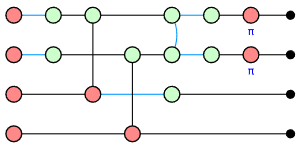
\includegraphics[width=0.5\textwidth]{figures/MS1.png}
    \end{figure}
    ZX diagram for the magic square game. First column and third row.
\end{frame}
\begin{frame}
    \begin{figure}
        \centering
        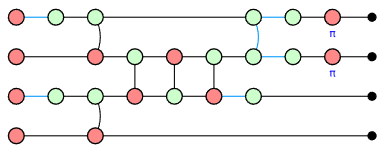
\includegraphics[width=0.5\textwidth]{figures/MS3.png}
    \end{figure}
    ZX diagram with connectivity constraints for the magic square game. First column and third row.
\end{frame}
\begin{frame}
    \begin{figure}
        \centering
        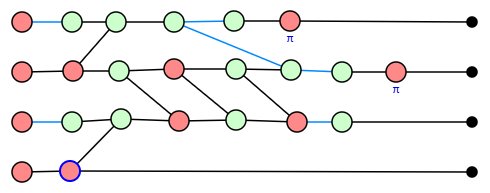
\includegraphics[width=0.5\textwidth]{figures/MS4.png}
    \end{figure}
    ZX diagram with explicit time ordering for the magic square game. First column and third row.
\end{frame}
\begin{frame}
    \begin{figure}
        \centering
        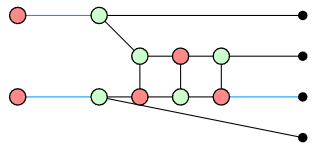
\includegraphics[width=0.5\textwidth]{figures/MS5.png}
    \end{figure}
    Simplified ZX diagram for the magic square game. First column and third row.
    \begin{table}
    \centering
    \resizebox{12cm}{!}{%
    \begin{tabular}{lccccccccc} 
        \toprule
        \textbf{Metric} & \textbf{(0,0)} & \textbf{(0,1)} & \textbf{(0,2)} & \textbf{(1,0)} & \textbf{(1,1)} & \textbf{(1,2)} & \textbf{(2,0)} & \textbf{(2,1)} & \textbf{(2,2)} \\
        \midrule
        Original Depth & 7  & 6  & 8  & 7  & 6  & 8  & 8  & 8  & 8  \\
        Original Pathwidth & 6 & 6 & 6 & 6 & 6 & 6 & 6 & 6 & 7 \\
        Optimized Depth & 5 & 6 & 6 & 6 & 6 & 6 & 6 & 6 & 7 \\
        Optimized Pathwidth & 5 & 5 & 6 & 5 & 5 & 6 & 6 & 6 & 6 \\
        \bottomrule
    \end{tabular}%
    }
    \end{table}
\end{frame}

\begin{frame}[allowframebreaks]{References}
    \printbibliography
\end{frame}

\end{document}